\documentclass[letterpaper, 10pt]{article}

\usepackage[colorlinks=true, allcolors=blue]{hyperref}
\usepackage{apacite}
\usepackage{amsmath}
\usepackage{tikz, tabularx}
\usetikzlibrary{arrows, fit,positioning}
\usepackage{fancyvrb}

\usepackage{setspace}
	\onehalfspacing

\author{George Vega Yon\thanks{gvega at spensiones.cl. Thanks to Damian C. Clarke, F\'elix Villatoro and Eduardo Fajnzylber and the Research team of the Chilean Pension Supervisor for their valuable contributions. The usual disclaimers applies.}\\Research Department\\Chilean Pension Supervisor}

\title{Introducing PARALLEL: Stata Module for Parallel Computing [draft]}

\date{This version September 26, 2012}

\begin{document}

\maketitle

\begin{abstract}
Inspired in the R library ``snow'' and to be used in multicore CPUs, {\tt parallel}
implements parallel computing methods through an OS's shell scripting (using
Stata in batch mode) to accelerate computations. By splitting the dataset into
a determined number of clusters this module repeats a task simultaneously over
the data-clusters, allowing to increase efficiency between two and five times,
or more depending on the number of cores of the CPU. Without the need of StataMP,
{\tt parallel} is, to the author's knowledge, the first user contributed Stata
module to implement parallel computing.
\end{abstract}

{\footnotesize 
\begin{description}
\item[Keywords:] Parallel Computing, High Performance Computing, Simulation Methods, CPU
\item[JEL Codes:] C87, C15, C61
\end{description}
}

\clearpage

\section{Introduction}

Currently home computers are arriving with extremely high computational capabilities. Multicore CPUs, standard in today's industry, expand the boundaries of productivity for the so called multitasking-users. Motivated by the video games industry, manufacturers have forged a market for low-cost processing units with the number-crunching horsepower comparable to that of a small supercomputer \cite{aldrich2011}.

In the same way, data availability has improved in a significant manner. Big-Data is an active topic by computer scientists and policy-makers considering the number of open-data initiatives taking place around the globe giving access to administrative data. Resources that, despite being available to researchers and policy makers, have not been exploited as they should.

The limited use of these social data resources is not a coincidence. As Gary King states in \citeA{King11022011}, issues involving privacy, standardized management and lack of statistical computing tools are still unsolved both for social scientists, and policy-makers. {\tt parallel} aims to make a contribution to these issues.

\section{Parallel Computing}

In simple terms, parallel computing is the simultaneous use of multiple compute resources to solve a computational problem \cite{barney2012parallel}. Parallelism can take place through several levels starting from (a) bit level, (b) instruction level, (c) data level and up to (d) task level. {\tt parallel} uses data level parallelism, which basically consists in simultaneously repeating an instruction over independent groups of data.

Using parallel computing allows the user to drastically decrease the time required to complete a computational problem. This is especially important for data scientists such as empirical economists and econometricians, given that in this way it is possible to implement algorithms characterized by a large number of calculations or, in the case of Stata, code interpretation such as flow-control statements like loops.

Flynn's taxonomy classification  provides a simple way to classify the type of parallelisms that researchers may require. Based on the type of instruction and the type of data, both of which can be single or multiple, Flynn identifies four classes of computer architectures \cite{barney2012parallel}.

\begin{table}[h]
\centering
\caption{Flynn's taxonomy\label{tab:flyntaxonomy}}
\begin{tabular}{lcc}
\hline
& Single Instruction & Multiple Instruction \\ \hline
Single Data & SISD & MISD \\
Multiple Data & SIMD & MIMD \\ \hline
\end{tabular}
\end{table}

According to this classification, {\tt parallel} would follow a Single Instruction Multiple Data (SIMD) design, where the parallelism takes place by repeating a single task over groups of data. Even though this is a very simple form of parallelism, significant improvements can be achieved from its use.

With regards to the size of the improvements, following Amdahl's law, the speed improvement $S$ depends upon (a) the proportion of potential de-serialization $P$; this is, the proportion of the algorithm that can be implemented in a parallel fashion, and (b) the number of fractions to be split, $N$.

\begin{equation}
S = \frac{1}{(1-P) + \frac{P}{N}}
\end{equation}

Thus, if $P$ tends to one, the potential speed gains $S$ will be equal to $N$. In the same way, as $P$ approaches to zero, any parallelization attempt will be worthless\footnote{A good technical review on modern themes on parallel computing is provided by \citeA{hill2008amdahl}}. Considering this, theoretically, SIMD class may reach perfect scaling.

\section{Parallel Computing in Econometrics}

Even though parallel computing is not a new idea\footnote{Applied sciences, physics, computer science and industry have taken considerable advantage of it.}, economics has drawn relatively little from parallel computing. In \citeA{Doornik2004} efforts are made by introducing a new C library based on matrix programming language Ox with the objective to promote parallel computing in social sciences. Using alternative approach, and after experimenting with GPU based parallel computing, \citeA{aldrich2011} show that using this approach to solve a Real Business Cycle model and using a consumer level NVIDIA video card, it is possible to reach speed improvements of around two hundred times, with this being a lower bound.

Statistical packages are also advancing in this line. Matlab provides its own Parallel Computing Toolbox\footnote{\url{http://www.mathworks.com/products/parallel-computing/}} which makes it possible to implement parallel computing methods through multicore computer, GPUs and computer clusters. GNU open-source R also has several libraries to implement parallel computing algorithms such as parallel, snow, and so forth\footnote{For more details see CRAN Task View on High-Performance and Parallel Computing With R \url{http://cran.r-project.org/web/views/HighPerformanceComputing.html}}. And Stata with its Multi-Processor edition, StataMP, implementing bit level parallelization makes it possible to achieve up to (or greater than) constant scale speed improvements \cite{stata2010}.

\section{PARALLEL: Stata module for parallel computing}

Inspired by the R library ``snow'' and to be used in multicore CPUs, {\tt parallel} implements parallel computing methods through OS's shell scripting (using Stata in batch mode) to speedup computations by splitting the dataset into a determined number of clusters\footnote{It is important to distinguish between two different ways to understand a cluster. In computer science a \emph{cluster}, or \emph{computer cluster}, refers to a set of computers connected so that they to work as a single system. Here, in the other hand, as this module is intended to be use by statisticians and social scientist in general, I refer to a cluster as a package of data which in this case does not necessary contains related observations (clustered).} in such a way to implement a data parallelism algorithm.

As exposed in \autoref{fig:howitworks}, right after {\tt parallel} splits the dataset into $n$ clusters it starts $n$ new independent stata instances in batch mode over which the same task is simultaneously executed. By default all the loaded instance globals and, optionally, programs and mata objects/programs are passed through. After every cluster stops the resulting datasets are appended and returned to the current stata instance without modifying other elements.

\begin{figure}[tp]
\centering
\caption{How {\tt parallel} works\label{fig:howitworks}}
\bigskip
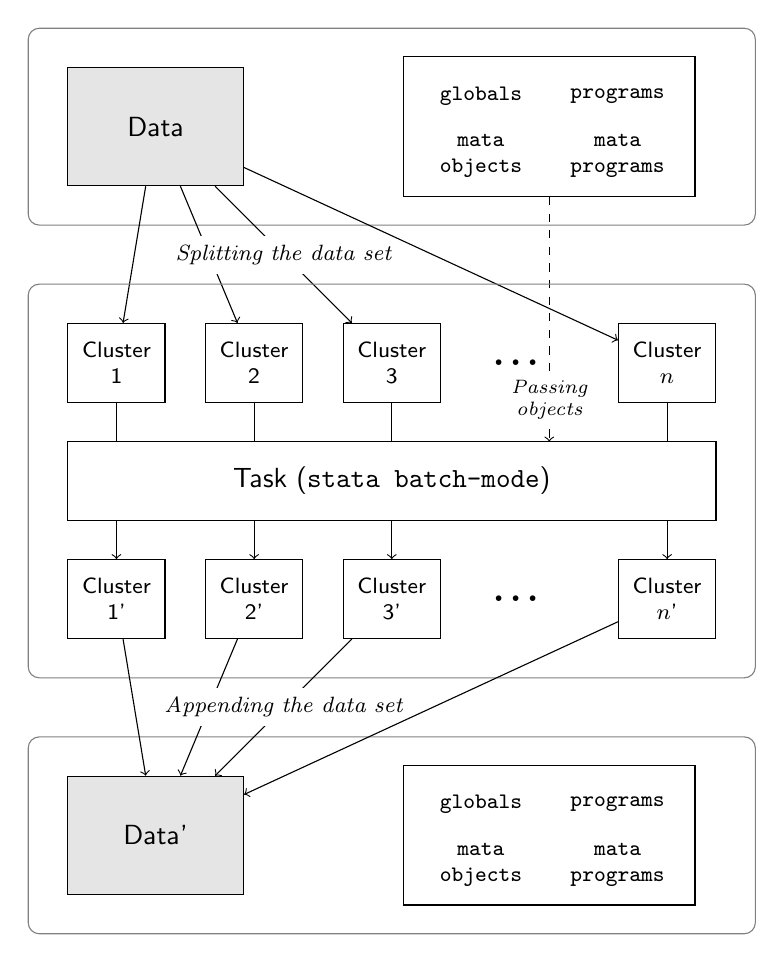
\begin{tikzpicture}[
	every node/.style={node distance=.5cm and .5cm, font=\sffamily}, 
	datablock/.style={rectangle, draw, fill=black!10, text width=2cm, minimum height=1.5cm, text badly centered},
	cluster/.style={rectangle, draw,text width=1cm, text badly centered, minimum height=1cm, font=\footnotesize\sffamily},
	explain/.style={rectangle, text width=5.5cm, align=left, font=\footnotesize\sffamily, node distance=.3, scale=.9}
	] 
	
\node [rectangle, draw=gray, text width=9cm, minimum height=2.5cm, rounded corners] (stata instance0) at (0,0) {};

% Original data
\node [datablock] (data) at (-3,0) {Data};
\matrix [
	draw=black,
	nodes={
		rectangle, text width=1.5cm, minimum height=.75cm, 
		scale=1,
		font=\tt\footnotesize, text badly centered}, column sep=0, row sep=0
	] (others) at (2,0) {
	\node {globals};& \node {programs}; \\
	\node {mata objects}; & \node {mata programs}; \\
};

% Data clusters
\node [cluster] (cluster3) at (0,-3) {Cluster 3};
\node [cluster, left=of cluster3] (cluster2) {Cluster 2};
\node [cluster, left=of cluster2] (cluster1) {Cluster 1};
\node [rectangle, right=of cluster3, text width=1cm, font=\Huge] (threepoints) {...};
\node [cluster, right=of threepoints,text badly centered] (clustern) {Cluster $n$};

% Splitting
\draw[->] (data) -- (cluster1);
\draw[->] (data) -- (cluster2);
\draw[->] (data) -- node [fill=white, font=\footnotesize\it] {Splitting the data set} (cluster3);
\draw[->] (data) -- (clustern);

\draw[->, dashed] (others) -- node [fill=white, font=\scriptsize\it, below=.65cm, text width=1.2cm, minimum height=.7cm,text badly centered] {Passing objects} (2,-4);

% Procesed clusters
\node [cluster] (cluster3p) at (0,-6) {Cluster 3'};
\node [cluster, left=of cluster3p] (cluster2p) {Cluster 2'};
\node [cluster, left=of cluster2p] (cluster1p) {Cluster 1'};
\node [rectangle, right=of cluster3p, text width=1cm, font=\Huge] (threepointsp) {...};
\node [cluster, right=of threepointsp,text badly centered] (clusternp) {Cluster $n$'};

\draw[->] (cluster1) -- (cluster1p);
\draw[->] (cluster2) -- (cluster2p);
\draw[->] (cluster3) -- (cluster3p);
\draw[->] (clustern) -- (clusternp);

% Task
\node [rectangle, draw=gray, text width=9cm, minimum height=5cm, rounded corners] (stata batch) at (0,-4.5) {};
\node [rectangle, fill=white, draw, text width=8cm, text badly centered,minimum height=1cm] (task) at (0,-4.5) {Task (\texttt{stata batch-mode})};

% Result
\node [rectangle, draw=gray, text width=9cm, minimum height=2.5cm, rounded corners] (stata instance1) at (0,-9) {};
\node [datablock] (datap) at (-3,-9) {Data'};
\matrix [
	draw=black,
	nodes={
		rectangle, text width=1.5cm, minimum height=.75cm, 
		scale=1,
		font=\tt\footnotesize, text badly centered}, column sep=0, row sep=0
	] (othersp) at (2,-9) {
	\node {globals};& \node {programs}; \\
	\node {mata objects}; & \node {mata programs}; \\
};

\draw[->] (cluster1p) -- (datap);
\draw[->] (cluster2p) -- (datap);
\draw[->] (cluster3p) -- node [fill=white, font=\footnotesize\it] {Appending the data set} (datap);
\draw[->] (clusternp) -- (datap);

% Text
%\node [explain, right=of stata instance0] {Starting (current) {\tt stata} instance loaded with data plus user defined {\tt globals}, {\tt programs}, {\tt mata objects} and {\tt mata programs}};

%\node [explain, right=of stata batch] {A new {\tt stata} instance (batch-mode) for every data-clusters. Programs, globals and mata objects/programs are passed to them.\\\bigskip The same algorithm (task) is simultaneously applied over the data-clusters.\\\bigskip After every instance stops, the data-clusters are appended into one.};

%\node [explain, right=of stata instance1] {Ending (resulting) {\tt stata} instance loaded with the new data.\\\bigskip User defined {\tt globals}, {\tt programs}, {\tt mata objects} and {\tt mata programs} remind unchanged.};

\end{tikzpicture}

\end{figure}

\pagebreak

The number of efficient computing clusters depends upon the number of physical cores (CPUs) with which your computer is built, e.g. if you have a quad-core computer, the correct cluster setting should be four. In the case of simultaneous multithreading, such as that from Intel's hyper-threading technology (HTT), setting {\tt parallel} following the number of processors threads, as it was expected, hardly results into a perfect speedup scaling. In spite of it, after several tests on HTT capable architectures, the results of implementing {\tt parallel} according to the machines physical cores versus its logicals shows small though significant differences.

{\tt parallel} is especially handy when it comes to implementing loop-based simulation models (or simply loops), Stata commands such as reshape, or any job that (1) can be repeated through data-blocks, and (2) routines that processes big datasets.

In the case of (pseudo) random number generation, {\tt parallel} allows to set one seed per cluster with the option {\tt seeds(\it{numlist}}).

At this time {\tt parallel} has been successfully tested in Windows and Unix machines. Tests using Mac OS are still pending.

\subsection{Syntax}

{\tt parallel}'s simplistic syntax is one of its key features. In order to use it, only two commands needed be entered: {\tt parallel setclusters}, which tells {\tt parallel} how many blocks of data are to be built (and thus how many Stata batch mode instances are needed to be run), and {\tt parallel do} (to run a do-file in parallel) or {\tt parallel:} (to use it as a prefix to parallelize a command). More, detailed, as specified in its help-file:

Setting the number of clusters (blocks of data)

\begin{verbatim}
parallel setclusters #
\end{verbatim}

Parallelizing a dofile

\begin{Verbatim}[commandchars=\\\{\}]
parallel do filename [,\emph{options}]
\end{Verbatim}

Parallelizing a stata command

\begin{Verbatim}[commandchars=\\\{\}]
parallel [, \emph{options}]:  stata_cmd
\end{Verbatim}

Parallel bootstrapping

\begin{Verbatim}[commandchars=\\\{\}]
parallel bs [, expression(exp) \emph{options}]:  stata_cmd
\end{Verbatim}

Parallel simulations

\begin{Verbatim}[commandchars=\\\{\}]
parallel sim , reps(#) [expression(exp) \emph{options}]:  stata_cmd
\end{Verbatim}

Removing auxiliary files

\begin{Verbatim}[commandchars=\\\{\}]
parallel clean [\emph{parallelid}]
\end{Verbatim}

\section{Results}
\def\win1{Intel Core i5 M560 (dual-core)}
\def\unix1{Intel Xeon X470 (octa-core)}

In what follows, I present some results testing the efficiency of {\tt parallel} over different hardware and software configurations using StataSE. The tables summarize the results. The first row presents the time required to complete the task using a single processor (cluster or thread as a computer scientist may prefer). The second line shows the total time spent to complete the task using {\tt parallel}, while the following three distinguish between setup (time taken to prepare the algorithm), compute (execution time of the task as such) and finish (mainly appending the datasets). Finally the last two show the ratio of CPU time over compute and total time respectively. Every time measure is presented in seconds.

It is important to consider that both setup time and finishing time increases as the problem size scales up.

All the test were performed checking whether if the parallel implementation returned different results from the serial implementation.

\subsection{Serial replacing using a loop}

This first test consists on, after a generation of $N$ pseudo-random values, using stata's {\tt rnormal()} function, replacing each and every one of the observations in a serial way (loop) starting from 1 to $N$. The observation's variable was replaced using the PDF of the normal distribution.

\begin{equation}
f(x) = \frac{1}{\sqrt{2\pi}}e^{\frac{-x^2}{2}}
\end{equation}

The code to be parallelized is

\begin{Verbatim}[tabsize=4, fontsize=\footnotesize]
--------------- begin of do-file -------------
local size = _N

forval i=1/`size' {
   qui replace x = 1/sqrt(2*`c(pi)')*exp(-(x^2/2)) in `i'
}
--------------- end of do-file ---------------
\end{Verbatim}

\noindent which is contained inside a do-file named ``myloop.do'', and can be executed through four clusters with {\tt parallel} as it follows

\begin{Verbatim}[tabsize=4, fontsize=\footnotesize]
parallel setclusters 4

parallel do myloop.do
\end{Verbatim}

This algorithm was repeated over 

\begin{equation*}N \in \{10,000; 100,000; 1,000,000; 10,000,000\}\end{equation*}

\begin{table}[!h]
\centering
\caption{Serial replacing using a loop on a Windows Machine (2 clusters)}
\begin{tabular}{l*{4}{c}}\hline
& \multicolumn{4}{c}{Problem Size} \\
& 10.000 &           100.000 &          1.000.000 &         10.000.000 \\ \hline
CPU &     0.12 &      1.22 &     11.72 &     58.03 \\
Total &     0.81 &      1.53 &      7.96 &     36.13 \\
\hspace{2mm} Setup &     0.02 &      0.08 &      0.56 &      2.86 \\
\hspace{2mm} Compute &     0.55 &      1.20 &      7.10 &     32.65 \\
\hspace{2mm} Finish &     0.25 &      0.25 &      0.30 &      0.62 \\
\hline Ratio (compute) &     0.23 &      1.01 &      1.65 &      1.78 \\
Ratio (total) &     0.15 &      0.80 &      1.47 &      1.61 \\
\hline
\multicolumn{4}{l}{\footnotesize Tested on an \win1 machine}
\end{tabular}
\end{table}

\begin{table}[!h]
\centering
\caption{Serial replacing using a loop on a Linux Server (4 clusters)\label{tab:serialreplace_linux}}
\begin{tabular}{l*{4}{c}}\hline
& \multicolumn{4}{c}{Problem Size} \\
& 10.000 &           100.000 &          1.000.000 &         10.000.000 \\ \hline
CPU &     0.25 &      1.79 &     17.64 &    176.16 \\
Total &     0.45 &      1.00 &      5.14 &     42.61 \\
\hspace{2mm} Setup &     0.02 &      0.11 &      0.81 &      5.16 \\
\hspace{2mm} Compute &     0.23 &      0.67 &      3.86 &     35.98 \\
\hspace{2mm} Finish &     0.21 &      0.23 &      0.46 &      1.47 \\
\hline Ratio (compute) &     1.13 &      2.68 &      4.57 &      4.90 \\
Ratio (total) &     0.56 &      1.79 &      3.43 &      4.13 \\
\hline
\multicolumn{5}{l}{\footnotesize Tested on an \unix1 machine}
\end{tabular}
\end{table}

\pagebreak

\subsection{Reshaping a large database}

Reshaping a large database is always a time consuming task. This example shows the execution of Stata's {\tt reshape wide} command for a large administrative dataset which contains unemployment insurance solicitations made by its users, i.e. a panel dataset.

The task was repeated over different sample sizes 
\begin{equation*}N \in \{1,000; 10,000; 100,000; 1,000,000; 10,000,000\}\end{equation*}

Using {\tt parallel} prefix syntax, the command is as it follows

\begin{Verbatim}[tabsize=4, fontsize=\footnotesize]
parallel, by(numcue) force:reshape wide ///
    tipsolic rutemp opta derecho ngiros, i(numcue) j(tiempo)
\end{Verbatim}

\noindent where the options {\tt by} consider observations grouping in so as not to split in between and {\tt force}, jointly used with {\tt by}, tells {\tt parallel} not to check whether if the dataset is actually sorted by, in this case, {\tt numcue}.

\begin{table}[!h]
\centering
\caption{Reshaping wide a large database on a Windows Machine (2 clusters)}
\begin{tabular}{l*{3}{c}}\hline
& \multicolumn{3}{c}{Problem Size} \\
& 100000 &         1000000 &         2000000 \\ \hline
CPU &     4.95 &     48.03 &    101.38 \\
Total &     5.04 &     39.58 &     81.40 \\
\hspace{2mm} Setup &     0.23 &      1.15 &      1.92 \\
\hspace{2mm} Compute &     4.34 &     34.96 &     72.14 \\
\hspace{2mm} Finish &     0.47 &      3.46 &      7.35 \\
\hline Ratio (compute) &     1.14 &      1.37 &      1.41 \\
Ratio (total) &     0.98 &      1.21 &      1.25 \\
\hline
\multicolumn{4}{l}{\footnotesize Tested on an \win1 machine}
\end{tabular}
\end{table}

\begin{table}[!h]
\centering
\caption{Reshaping wide a large database on a Windows Machine (4 clusters with HTT)}
\begin{tabular}{l*{3}{c}}\hline
& \multicolumn{3}{c}{Problem Size} \\
& 100000 &         1000000 &         2000000 \\ \hline
CPU &     4.91 &     50.48 &    106.03 \\
Total &     4.42 &     29.00 &     69.69 \\
\hspace{2mm} Setup &     0.45 &      2.06 &      3.51 \\
\hspace{2mm} Compute &     3.84 &     23.57 &     55.86 \\
\hspace{2mm} Finish &     0.13 &      3.37 &     10.31 \\
\hline Ratio (compute) &     1.28 &      2.14 &      1.90 \\
Ratio (total) &     1.11 &      1.74 &      1.52 \\
\hline
\multicolumn{4}{l}{\footnotesize Tested on an \win1 machine}
\end{tabular}
\end{table}

\begin{table}[!h]
\centering
\caption{Reshaping wide a large database on a Linux Server (4 clusters)}
\begin{tabular}{l*{3}{c}}\hline
& \multicolumn{3}{c}{Problem Size} \\
& 100.000 &          1.000.000 &         5.000.000 \\ \hline
CPU &     9.00 &    101.94 &    564.13 \\
Total &     4.41 &     43.92 &    317.60 \\
\hspace{2mm} Setup &     0.77 &      1.43 &     10.03 \\
\hspace{2mm} Compute &     3.17 &     38.52 &    283.05 \\
\hspace{2mm} Finish &     0.47 &      3.98 &     24.53 \\
\hline Ratio (compute) &     2.84 &      2.65 &      1.99 \\
Ratio (total) &     2.04 &      2.32 &      1.78 \\
\hline
\multicolumn{4}{l}{\footnotesize Tested on an \unix1 machine}
\end{tabular}
\end{table}

\begin{table}[!h]
\centering
\caption{Reshaping wide a large database on a Linux Server (8 clusters)}
\begin{tabular}{l*{3}{c}}\hline
& \multicolumn{3}{c}{Problem Size} \\
& 100000 &         1000000 &         5000000 \\ \hline
CPU &     9.21 &     98.87 &    534.34 \\
Total &     3.95 &     47.08 &    233.90 \\
\hspace{2mm} Setup &     0.94 &      2.63 &     18.37 \\
\hspace{2mm} Compute &     2.46 &     40.13 &    188.47 \\
\hspace{2mm} Finish &     0.55 &      4.32 &     27.07 \\
\hline Ratio (compute) &     3.74 &      2.46 &      2.84 \\
Ratio (total) &     2.33 &      2.10 &      2.28 \\
\hline
\multicolumn{4}{l}{\footnotesize Tested on an \unix1 machine}
\end{tabular}
\end{table}

\pagebreak

\subsection{Extended test: Monte Carlo Simulation}

In \citeA{baum2007} a simple Monte Carlo experiment is perform which simulates the performance of a estimator of sample mean, $\bar x$, in a context of heteroskedasticity. The model to be

\begin{equation}
y_i = \mu + \epsilon_i \sim N(0,\sigma^2)
\end{equation}

Let $\epsilon$ be a $N(0,1)$ variable multiplied by a factor $cz_i$, where $z_i$ varies over $i$. We will vary parameter $c$ between 0.1 and 1.0 and determine its effect on the point and interval estimates of $\mu$; as a comparison, we will compute a second random variable which is homoskedastic, with the scale factor equalling $c\bar z$.

From web dataset {\tt census2} the variables {\tt age}, {\tt region} (which can be 1, 2, 3 or 4) and the mean of {\tt region} are used as $\mu$, $z_i$ and $\bar z$ respectively.

The simulation program, stored in ``mcsimul1.ado'', is defined as
\bigskip

\begin{Verbatim}[tabsize=4, fontsize=\footnotesize]
--------------- begin of ado-file ------------
program define mcsimul1, rclass
	version 10.0
	syntax [, c(real 1)]
	
	tempvar e1 e2
	gen double `e1'=invnorm(uniform())*`c'*zmu
	gen double `e2'=invnorm(uniform())*`c'*z_factor
	
	replace y1 = true_y + `e1'
	replace y2 = true_y + `e2'
	
	summ y1
	return scalar mu1 = r(mean)
	return scalar se_mu1 = r(sd)/sqrt(r(N))
	
	summ y2
	return scalar mu2 = r(mean)
	return scalar se_mu2 = r(sd)/sqrt(r(N))
	
	return scalar c = `c'
end
--------------- end of ado-file --------------
\end{Verbatim}
\bigskip

In what is next, the do-file that runs the simulation, stored as ``montecarlo.do'', it is compound of two parts: (a) setting the iteration range by which $c$ is going to vary, and (b) looping over the selected range. For the first part the do-file uses the local macro {\tt pll\_instance} which is the numer of the parallel stata instance running, thus there are as many as clusters have been declared, number available with the global macro {\tt PLL\_CLUSTERS}. This way, if the macro {\tt PLL\_CLUSTERS} equals two and the macro {\tt pll\_instance} equals une, then the range will be defined from one to five\footnote{Note that if the local macro {\tt pll\_id}, which contains a special random number that identifies an specific {\tt parallel} run (more details in its help file), length is zero it means that the do-file is not running in parallel mode, thus it is been executed in a serial way where the loop range starts from one to ten.}.
\bigskip

\begin{Verbatim}[tabsize=4, fontsize=\footnotesize]
--------------- begin of do-file -------------
// Defining the loop range
local num_of_intervals = 10
if length("`pll_id'") == 0 {
	local start = 1
	local end = `num_of_intervals'
}
else {
	local ntot = floor(`num_of_intervals'/$PLL_CLUSTERS)
	local start = (`pll_instance' - 1)*`ntot' + 1
	local end = (`pll_instance')*`ntot'
	if `pll_instance' == $PLL_CLUSTERS local end = 10
}

local reps 1000

// Loop
forval i=`start'/`end' {
	qui webuse census2, clear
	gen true_y = age
	gen z_factor = region
	sum z_factor, meanonly
	scalar zmu = r(mean)
	qui {
		gen y1 = .
		gen y2 = .
		local c = `i'/10
		set seed `c'
		simulate c=r(c) mu1=r(mu1) se_mu1 = r(se_mu1) ///
				mu2=r(mu2) se_mu2 = r(se_mu2), /// 
				saving(cc`i', replace) nodots reps(`reps'): ///
				mcsimul1, c(`c')
	}
}
--------------- end of do-file ---------------
\end{Verbatim}
\bigskip

\noindent This do-file will be executed from stata using {\tt parallel do} syntax. As there is no need of splitting any dataset (these are loaded every time that the main {\tt loop\_simul.do}'s loop runs), we add the option {\tt nodata}. This way the main do-file will look like this
Finally, the do-file from which parallel runs the simulation
\bigskip

\begin{Verbatim}[tabsize=4, fontsize=\footnotesize]
--------------- begin of do-file -------------
clear all
parallel setclusters 5
parallel do loop_simul.do, nodata
--------------- end of do-file ---------------
\end{Verbatim}
\bigskip

By this {\tt parallel} will start, in this case, five new independent stata instances, each one looping over the ranges 1/2, 3/4, 5/6, 7/8 and 9/10 respectively.

Most of the code has been exactly copied with the exception of the addition of a new code line {\tt set seed}. In order to be able to compare both serial and parallel implementations of the algorithm it was necessary to set a particular seed for each loop, inside ``montecarlo.do'' right before {\tt simulate} command.

\begin{table}[!h]
\centering
\caption{Monte Carlo Experiment on a Windows Machine}
\begin{tabular}{l*{2}{c}}\hline
& \multicolumn{2}{c}{Number of Clusters} \\
& 2 &               4 \\ \hline
CPU &    28.50 &     28.92 \\
Total &    17.49 &     18.30 \\
\hspace{2mm} Setup &     0.11 &      0.12 \\
\hspace{2mm} Compute &    17.27 &     18.07 \\
\hspace{2mm} Finish &     0.11 &      0.11 \\
\hline Ratio (compute) &     1.65 &      1.60 \\
Ratio (total) &     1.63 &      1.58 \\
\hline
\multicolumn{3}{c}{\footnotesize Tested on a \win1 machine}
\end{tabular}
\end{table}

\begin{table}[!h]
\centering
\caption{Monte Carlo Experiment on a Linux Server}
\begin{tabular}{l*{3}{c}}\hline
& \multicolumn{3}{c}{Number of Clusters} \\
& 2 &               3 &               5 \\ \hline
CPU &    40.97 &     39.01 &     36.44 \\
Total &    18.35 &     15.20 &      7.62 \\
\hspace{2mm} Setup &     0.11 &      0.11 &      0.12 \\
\hspace{2mm} Compute &    18.13 &     14.99 &      7.41 \\
\hspace{2mm} Finish &     0.10 &      0.10 &      0.10 \\
\hline Ratio (compute) &     2.26 &      2.60 &      4.92 \\
Ratio (total) &     2.23 &      2.57 &      4.78 \\
\hline
\multicolumn{4}{c}{\footnotesize Tested on a \unix1 machine}
\end{tabular}
\end{table}

\pagebreak

\section{Concluding Remarks}

As stated by computer scientist Ph.D. Wen-Mei Hwu\footnote{Chief Scientist at \emph{Parallel Computing Institute} \url{http://parallel.illinois.edu/news-and-media/gpus-path-future}}, parallel computing is the future of supercomputing, and giving the computer industry's fast pace of development, scientists in various areas are making real efforts to promote its usage. In spite of this, many of social scientist do not work with it due to its lack of user-friendly implementations.

In the case of Stata, {\tt parallel} is, to the authors knowledge, the first public user-contribution to parallel computing. The major benefits, measured in terms of speedups, can be reached by simulation models and non-vectorized operations such as control-flow statements. Speed gains are directly related to the proportion of the algorithm that can be de-serialized and the number of processors with which the parallelization is made, making possible reach near to constant scale improvements.

Notwithstanding the simplicity of this type of parallelism, giving to its easy way, it seems like a worthy activity for a wide range of social scientists and researchers.

\nocite{tierney2012,r}
\bibliographystyle{apacite}
\bibliography{bib}

\end{document}
